\section{Décomposition du logiciel et structures de communication}

\subsection{Architecture modulaire}

Le projet MiniJAJA a été conçu selon une architecture modulaire respectant le principe de séparation des responsabilités. Cette organisation permet une indépendance des composants et facilite la maintenance et l'évolution du système.

\subsubsection{Les modules principaux}

Le système est décomposé en quatre modules distincts, chacun responsable d'une partie spécifique du processus de compilation et d'interprétation :

\paragraph{Module LexerParser}
Ce module constitue le point d'entrée de l'analyse du code source MiniJaja. Il assure la transformation du texte source en une représentation structurée exploitable. Utilisant ANTLR4, il produit d'abord un Concrete Syntax Tree (CST) qui est ensuite converti en Abstract Syntax Tree (AST). Ce module expose des interfaces permettant aux autres composants d'accéder à la représentation abstraite du programme sans dépendre des détails d'implémentation du parseur.

\paragraph{Module Mémoire}
Le module Mémoire implémente le modèle d'exécution à base de Pile et de Tas (Stack/Heap). Il encapsule la gestion de la Table des Symboles, l'allocation dynamique sur le Tas via le système Buddy, et le mécanisme de ramasse-miettes par comptage de références. Ce module fournit une API claire pour les opérations de déclaration, d'affectation et de libération de variables, masquant ainsi la complexité des structures de données sous-jacentes.

\paragraph{Module Compiler}
Le module Compiler orchestre la chaîne de compilation complète. Il fait le lien entre le LexerParser (pour obtenir l'AST) et le générateur de code JajaCode. Il coordonne également l'analyse sémantique et la résolution des portées. Ce module expose des interfaces de haut niveau permettant de compiler un fichier source vers du code JajaCode, en gérant les éventuelles erreurs de compilation.

\paragraph{Module GUI}
Le module d'interface graphique (GUI) fournit l'environnement interactif pour l'utilisateur. Il intègre un éditeur de code avec coloration syntaxique, une console de sortie, un débogueur pas à pas et une visualisation de l'état de la mémoire. Ce module consomme les services exposés par les autres modules sans jamais manipuler directement les structures internes (AST, Pile, Tas).

\begin{figure}[h]
    \centering
    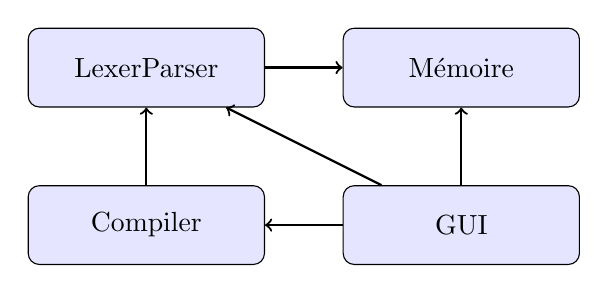
\begin{tikzpicture}[
        module/.style={rectangle, draw, rounded corners, minimum width=3cm, minimum height=1cm, text centered, fill=blue!10},
        arrow/.style={->, thick}
    ]
        \node[module] (lexer) at (0,0) {LexerParser};
        \node[module] (memoire) at (4,0) {Mémoire};
        \node[module] (compiler) at (0,-2) {Compiler};
        \node[module] (gui) at (4,-2) {GUI};

        \draw[arrow] (lexer) -- (memoire);
        \draw[arrow] (compiler) -- (lexer);
        \draw[arrow] (gui) -- (lexer);
        \draw[arrow] (gui) -- (memoire);
        \draw[arrow] (gui) -- (compiler);
    \end{tikzpicture}
    \caption{Architecture modulaire du projet MiniJAJA}
\end{figure}

\subsection{Structures de communication}

La communication entre modules repose sur des interfaces Java bien définies et des objets de transfert de données (DTO) garantissant le découplage.

\subsubsection{Interfaces Java}

Chaque module expose des interfaces publiques qui définissent son contrat avec les autres composants. Par exemple, le module Mémoire expose une interface \texttt{SymbolTable} permettant de déclarer et accéder aux symboles sans exposer l'implémentation interne de la table de hachage. De même, le LexerParser fournit une interface \texttt{Parser} qui garantit l'obtention d'un AST sans révéler les détails d'ANTLR.

\subsubsection{Objets de transfert (DTO)}

Les données échangées entre modules transitent via des objets immutables ou des structures de données standardisées. L'AST, par exemple, est composé de nœuds (Node) qui sont des structures de données pures sans logique métier. Cela permet au Compiler de manipuler l'arbre sans dépendre du module qui l'a produit.

\subsubsection{Événements et observateurs}

Le module GUI utilise le pattern Observer pour réagir aux changements d'état de l'interpréteur. Lorsque le débogueur avance d'une instruction, des événements sont émis permettant à l'interface de mettre à jour l'affichage de la mémoire et de la position dans le code sans couplage direct avec le moteur d'exécution.

\subsection{Gestion des dépendances Maven}

L'architecture modulaire est renforcée par la structure Maven multi-modules. Chaque module possède son propre \texttt{pom.xml} définissant ses dépendances. Le module GUI dépend des trois autres, mais LexerParser, Mémoire et Compiler peuvent être compilés et testés indépendamment. Cette organisation facilite les tests unitaires et permet un développement parallèle des différentes briques sans blocage.
